\chapter*{El proceso de ingesta}
\label{chap:ingesta}
\section*{Infraestructura}
Como ya hemos explicado, la naturaleza del proyecto implica obtener, procesar, transformar e integrar múltiples fuentes de datos. Con eso en mente, hemos ensamblado una infraestructura orientada a fuentes de datos. Esa infraestructura responde a varias necesidades:
\begin{itemize}
    \item \textbf{Escalabilidad} - las exigencias de memoria y procesamiento de nuestros flujos de extracción, transformación y carga (comúnmente llamados ETL, por sus siglas en inglés) pueden variar considerablemente con el tamaño de las bases de datos. Así, para datos como los padrones o cuestionarios largos sería óptimo correr 10 procesos en paralelo, mientras que para cuestionarios pequeños como CUAPS esa capacidad sería mal aprovechada.
    \item Portabilidad - es también importante que ningún proceso quede supeditado a ser ejecutado en una plataforma o sistema operativo en particular, para así disminuir las necesidades de mantenimiento del código.
    \item \textbf{Seguridad} - dado el tipo de información con el que contamos, debemos garantizar la seguridad y privacidad de los datos sin comprometer la flexibilidad de agregar nuevos colaboradores al proyecto de ser necesario.
    \item \textbf{Actualización periódica y eficiente} - al tener un flujo continuo de datos hacia nuestros modelos, necesitamos que esos procesos ETL puedan ser replicados sin mayor esfuerzo. Asimismo, queremos evitar que alguna tarea sea repetida innecesariamente.
    \item \textbf{Documentación} - para que pueda ser replicado con facilidad, es necesario que cualquier persona con acceso al código pueda entender el flujo de datos, la serie de procesos que deben ocurrir y las fuentes de datos necesarias para replicar el análisis.
\end{itemize}
Considerando estas necesidades, usamos varias partes móviles para el proceso de ETL. Todos nuestros procesos son ejecutados en un servidor de AWS EC2, que tiene montado un disco EBS para almacenamiento del código. En ese servidor se construye un contenedor de Docker a partir de una imagen privada con sistema operativo Linux Debian, que cuenta con Python, R y los paquetes necesarios para ejecutar el proyecto. La mayor parte de nuestras necesidades de almacenamiento de datos a través del flujo ETL se llevan a cabo en AWS S3, para al final escribirse a una base de datos AWS RDS en PostgreSQL. Por último, tenemos un registro del linaje de los datos en una base de datos orientada a grafos, en Neo4j.
\par
\noindent
Para facilitar la actualización periódica de los datos, todo el flujo está orquestado en Luigi con las tareas como sigue:
\par
\noindent
\begin{figure}[h]
    \caption{Flujo de datos}
    \centering
    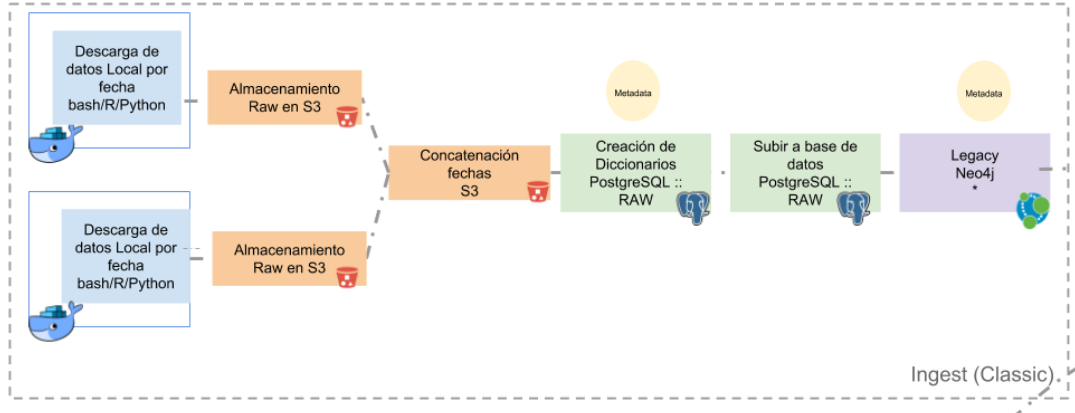
\includegraphics[width=\textwidth]{ingest_pipeline.png}
\end{figure}
Así, todas nuestras fuentes de datos son ingestadas concatenando el conjunto de datos históricos antes de escribirse a la base de datos. Cada fuente de datos tiene su propio script de ingesta local, escrito ya sea en \textit{bash, python} o \textit{R} que toma como parámetros la fecha del dato, el nombre de la fuente y la ruta de descarga local al servidor.
\section*{Scripts de ingesta}
Para ingestar los archivos de CUIS, es necesario utilizar los paquetes \textit{unzip} y \textit{unrar}\ref{unrar_debian, unzip_debian}, que permiten la descompresión de archivos, y \textit{csvkit} \ref{csvkit}, un paquete de \textit{python} con integración a \textit{bash} que permite aplicar distintas transformaciones a datos de tipo CSV, incluyendo la conversión a CSV desde archivos de Excel.
Todos los códigos de ingesta están disponibles en el \autoref{chap:apendice}.
